\paragraph{Real-World Traffic Experiment.}
\label{sec:real}
We complement the previous experiment with real-world trajectory data. We use the Porto Taxi Trajectory Dataset~\cite{pkdd_2015_339}. On this dataset, the number of samples is small enough that the conformal guarantee $\phi$ differs significantly on the held-out set compared to the compression parameter $\tau$, so that we are not in the ``uniform convergence'' regime. We show that the nested subgraph approach in Section~\ref{sec:fixed_optimal} achieves robust compression in this regime (in addition to providing a worst-case theoretical compression guarantee).

The dataset consists of 1.7 million taxi trajectories in Porto, Portugal. We define a bounding box around the Greater Porto area and discretize this region into a $100 \times 100$ grid. Each valid grid cell ($\approx 100m \times 100m$) containing at least one GPS reading constitutes a vertex in our hypergraph. Each taxi trip is mapped to the set of unique grid cells it traverses, forming a hyperedge.

We filter on trips from the airport to the city center, resulting in around $300$ trips. Using $k$-means clustering on trajectory midpoints, we identify two distinct route modes naturally taken by drivers: The trips that take highways that circle around the city and the trips that cut diagonally (likely taking city streets).  We construct a dataset with 40\% of the former and 60\% of the latter trajectories. We split the data randomly into 100 train and 100 disjoint test routes. We use the training data to find the LP and greedy solutions, and use the test data to evaluate coverage.

%We solve the LP on the training data for $\tau = 0.2, 0.4, 0.8, 0.99$, and round to select all non-zero variables, and as before, compute the coverage $\phi$ of the resulting solutions on the test paths. Figure~\ref{fig:porto_combined}(b) shows the number of edges used by the LP solution for different $\tau$ as bars, and plots the training and test coverage of the LP and Greedy solutions for this budget. 

\begin{figure*}[t]
    \centering
    % --- Subfigure (a): The Selection Maps ---
    \begin{subfigure}[b]{0.63\textwidth}
        \centering
        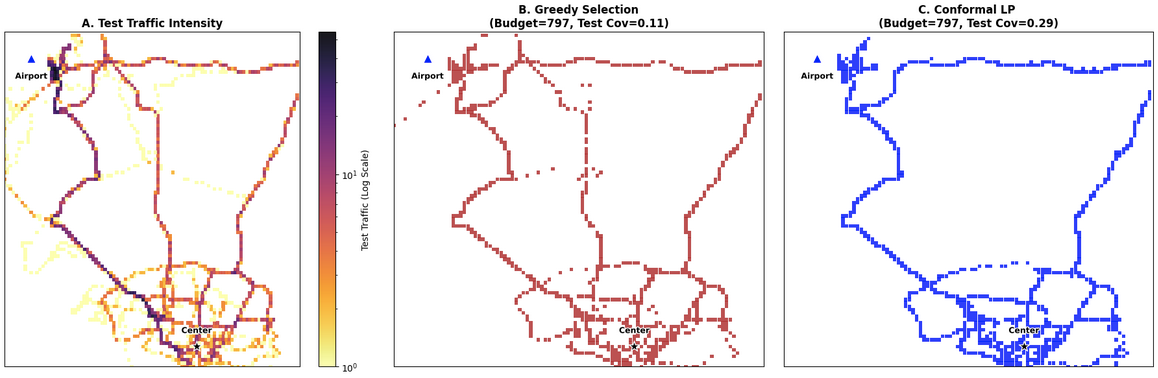
\includegraphics[width=\linewidth]{images/proto_conformal2.png} 
        \caption{\textbf{(Left)} Heatmap of test traffic. \textbf{(Center)} and {\bf (Right)}  Edge selection for Forward Greedy and LP respectively with the same edge budget of $797$ edges.}
        \label{fig:porto_visual}
    \end{subfigure}
    \hfill
    % --- Subfigure (b): Heatmap and Curve ---
    \begin{subfigure}[b]{0.35\textwidth}
        \centering
        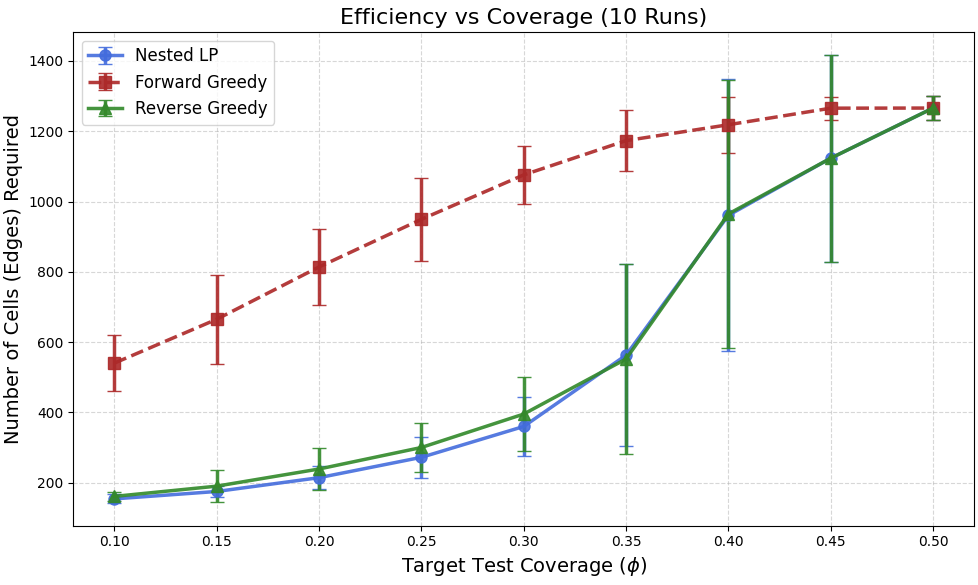
\includegraphics[width=\linewidth]{images/real_reverse_eff2.png} 
        \caption{Greedy and LP compression over $10$ runs. }
        \label{fig:porto_stats}
    \end{subfigure}
    \caption{Real-world validation on Porto Taxi data (Airport $\to$ Center).}
    \label{fig:porto_combined}
\end{figure*}

In Figure~\ref{fig:porto_combined}(b), we note that the LP and the reverse greedy algorithm achieve comparable and non-trivial compression for $\phi \le 0.4$ relative to the forward greedy baseline. Note in this case that the number of paths is not large enough to ensure a ``uniform convergence'' type behavior in the samples (as in Theorem~\ref{cor:efficiency}), so that the conformal guarantee even with no compression is $\phi \le 0.5$. Nevertheless, we observe that our algorithm provides robust compression in this regime. The edge selections when the LP and Forward Greedy procedures are allowed $797$ edges (corresponding to  $\tau = 0.8$ for the LP) are shown in Figure~\ref{fig:porto_combined}(a). In this setting, greedy  prioritizes an additional highway to the airport, while the LP prioritizes  the city center. 

One interesting observation is that reverse greedy and LP achieve comparable performance on this instance, suggesting that the empirical route distribution does not exhibit strong compressible structure beyond what is captured by frequency-based heuristics.  As mentioned before, our goal in this experiment is to demonstrate that the nested compression approach provides a strong compression guarantee even in the sparse sample regime where the conformal guarantee differs significantly from the $\tau$ used on the training samples. Furthermore, the LP rounding algorithm always provides a compression guarantee in the sense of Theorem~\ref{thm:main-det}, and as the example below shows, reverse greedy (or forward greedy) cannot provide such a guarantee in general.

\begin{example}
Fix some relaxation parameter $\kappa > 0$ as in Theorem~\ref{thm:main-det}. Choose some $\epsilon > 0$ so that $1+\kappa \le \frac{1-\epsilon}{\epsilon}$. There is a path $P$ with $a$ edges between $s$ and $t$ with $w_P = \epsilon$ fraction of traffic. In addition, there is a set $S$ of $b \ll a$ parallel edges between $s$ and $t$ each with $w = \frac{1-\epsilon}{b}$ fraction of traffic. Suppose the goal is to cover $\tau = 1-\epsilon$ fraction of traffic. Then the optimal solution deletes $P$ and incurs cost $b$ in terms of number of edges. Reverse greedy deletes edges from $S$ until the deleted coverage is $(1+\kappa) \cdot \epsilon$ and incur edge cost at least $a \gg b$, so that no worst-case compression guarantee analogous to Theorem~\ref{thm:main-det} is possible.
\end{example}
